\documentclass{acm_proc_article-sp}
\usepackage[utf8]{inputenc}
\usepackage{graphicx}
\usepackage{caption}
\usepackage{subcaption}
\usepackage{color}
\usepackage{amsmath}
%opening
\title{Fast online predictive compression of radio astronomy data}
\numberofauthors{1} 
\author{
% 1st. author
\alignauthor
Benjamin V. Hugo\\
       \affaddr{Department of Computer Science}\\
       \affaddr{University of Cape Town}\\
       \email{bennahugo@aol.com}
}
\begin{document}

\maketitle
\begin{abstract}
 {\color{red}TODO: add at end of writeup}
\end{abstract}

\section{Introduction}
In this report we will investigate the feasibility of compressing radio astronomy data using a predictive compression scheme. All compression techniques
build on the central concept of reducing redundant data. The exact definition of this redundancy is of course context dependent. It may take the form of 
repeated values, clustered values, wasteful encoding processes and many others. We also point out the difference between lossy and lossless compression, as
well as online versus offline compression.

In a lossless compression scheme the compression is completely invertible with \textit{no} loss of information after a decompression step is performed. Lossy
compression on the other hand discards unimportant data and gives much higher compression ratios than lossless methods. Lossy compression is useful in many
instances where subtle changes in data is not considered problematic. Some examples of this are the removal of high frequency data from images, sampling 
voice data at a lower rate than music or to employ a commonly used technique called \textit{quantization} where data is simply binned into consecutive ranges 
(or \textit{bins}).

An online compression scheme refers to a process of compressing data on-the-fly or as it is being transmitted on the wire. The results are sent off to subsequent 
processes such transmission over a network or storage to disk. This is in contrast to to an offline scheme where data is compressed as a separate process which doesn't
form part of the primary work flow of a system. An online process are normally considered to be fast enough as not to slow the overall data processing capabilities of 
a system.

We will measure compression performance both in terms of effectiveness through a compression ratio described below \cite[p. 10]{salomon2004data} and throughput speed. A 
compression ratio closer to 0 indicates a smaller output file and values greater than 1 indicates that the algorithm inflated the data instead of shrinking it.
\begin{equation}
 \text{Compression ratio} := \frac{\text{size of the output stream}}{\text{size of the input stream}}
\end{equation}
\begin{equation}
 \text{Throughput} := \frac{\text{input processed (in GB)}}{\text{difference in time (in seconds)}}
\end{equation}
We will now discuss the relevance of our problem and give a breakdown of the most commonly used compression techniques. We will then discuss a detailed design
of our predictive compression scheme, different implementation strategies along with technical details and a section with results and discussion.
\section{Background}
\subsection{KAT-7, MeerKAT and the SKA}
South Africa and Australia are the two primary hosting countries for the largest radio telescope array in the world, known as the Square Kilometer Array. 
The SKA will give astronomers the opportunity to capture very high resolution images, over a wide field of view, covering a wide range of frequencies ranging 
from 70 MHz to 10 GHz. Upon completion in 2024 the array will consist of around 3000 dishes in the high frequency range and thousands of smaller antennae to 
cover the low frequency band. The South African branch of the SKA will be completed in 3 main phases. Phase 1 is a fully operational prototype 7-dish array 
called the KAT-7. The second phase, known as the MeerKAT, will consist of approximately 90 dishes to be erected in the central Karoo. The final phase add 
the remaining dishes and increase the baseline of the telescope to roughly 3000 km.

Due to the high signal sampling rate it is expected that each of these dishes will produce data rates up to 420 GiB/s while the lower frequency aperture arrays 
will produce up to 16 TiB/s. These rates, coupled with the scale of the SKA, will require a processing facility capable of handling as much as 1 Petabyte of 
data every 20 seconds, necessitating the need for massive storage facilities. Innovative techniques are required to deal with this complex requirement of high 
throughput rates while effectively reducing the large storage requirements by means of data compression. Refer to fig.~\ref{MeerKAT_PIPELINE} for an overview of
the MeerKAT pipeline. Due to the limited scope of the project we propose that the compression step can be introduced as an additional step for each of the cluster
nodes, although it may be suitable for introduction on the Field Programmable Gate Arrays in further research.
\begin{figure}[h!]
 \centering
 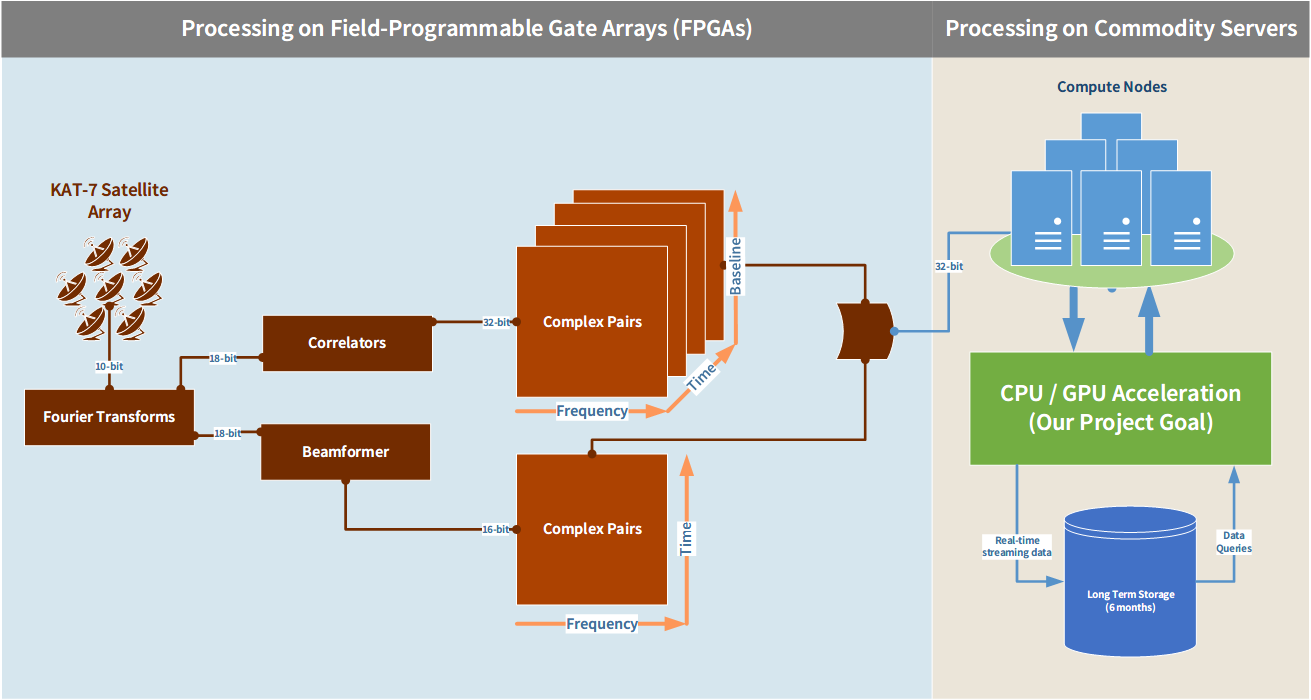
\includegraphics[width=0.50\textwidth]{Process.png}
 \caption{High-level overview of the MeerKAT pipeline}
 \label{MeerKAT_PIPELINE}
\end{figure}
\subsection{Overview of data compression techniques}
There are considered to be 4 broad categories of compression techniques \cite{salomon2004data}. These are some basic methods, Lempel-Ziv methods, statistical methods 
and transforms.
\subsubsection{Basic methods}
The more intuitive methods include commonly employed methods such as Run-Length Encoding (RLE) which, simply put encodes runs of characters using some reserved 
character and a number indicating the length of the run.

Another basic technique which is particularly relevant for application on numerical data a predictive compression scheme. Such a compression scheme encodes the 
difference between each predicted succeeding value and the actual succeeding value. This can be quite successfully employed to compress data generated from time series \cite{engelson2000lossless}.
\subsubsection{Lempel-Ziv methods}
Also commonly referred to as “LZ” or dictionary methods is a class of algorithms with many variants and is one of the more popular adaptive techniques in modern 
compression utilities. In their simplest form these methods normally uses both a search and a lookahead buffer to encode recurrent phrases using fixed-size codes. An 
adaptive compression technique is useful in circumstances where the probability distribution of the underlying dataset is not known in advance or may change over time. 
One example of such an LZ method is the GNU compression utility Gzip which implements the Deflate algorithm \cite[ch. 3]{salomon2004data}.
\subsubsection{Statistical methods}
This class of algorithms normally uses variable length codes to achieve an optimal (or near optimal) encoding of dataset. In information theory this optimal encoding is 
described as an entropy encoding. Entropy is the measurement of the information contained in a single base-n symbol (as transmitted per time unit by some source). Mathematically
redundancy is defined as follows ($n$ is the size of a symbol set and $P_{i}$ is the probability that a symbol $c_{i}$ is transmitted from a source)\cite[p. 46 - 47]{salomon2004data}:
\begin{equation}
 R := \log_2n + \sum_1^nP_i\log_2P_i
\end{equation}
As the name may suggest the techniques uses the probability of occurrence to assign shorter codes to frequently occurring values in order to eliminate redundancy. The 
class of statistical methods include two widely employed techniques known as Huffman and Arithmetic coding respectively. Huffman coding assigns shorter \textit{integral-length} codes, while arithmetic 
coding assigns \textit{real-length} subintervals of [0,1) to frequently occurring symbols \cite{Witten:1987:ACD:214762.214771}\cite[ch. 2]{salomon2004data}.

Both approaches lead to variable-size codes. Both techniques have adaptive versions which are useful in situations where the probability distributions change or have to be estimated. This 
approach is also applicable to the situation where the symbol table has to be computed on the fly, because it is impossible to perform multiple passes. Arithmetic coding is considered to approach 
a true entropy encoder and achieves higher compression ratios in both adaptive and non-adaptive cases. It should be pointed out that the decompression step of Arithmetic coding is slow and 
unsuitable for cases where fast access is required \cite{ray1995database,williams1999compressing}\cite[ch. 2]{salomon2004data}.

\subsubsection{Transforms}
As the name suggest it can be useful to transform a dataset from one form to another in order to exploit its features for the purposes of compression. Such transformations 
includes, for example, wavelet transforms. As the name suggests a wavelet is a small wave-like function that is only non-zero over a very small domain and can be used 
to represent, for example, the high frequency components in an image (JPEG2000 and DjVu are popular formats using wavelet transforms). The coefficients within this 
transformation can then be further compressed using other techniques, for example, Huffman coding. If lossy compression (loss of accuracy which cannot be recovered after 
decompression)  is tolerable, quantization can be used to discard unimportant values (for example the high frequency features of an image) \cite{952804}\cite[ch. 5]{salomon2004data}.

Transforms are furthermore particularly useful where multiple levels of detail are desired. An example of this may include the transfer of scientific data over a network 
for real-time analysis and observation. Low resolution samples can be constantly transferred, while higher resolution samples can be transferred upon request \cite{Tao:1994:PTS:951087.951108}.
\subsection{IEEE 754}
The IEEE 754 standard of 2008 defines 3 interchange formats (32-bit, 64-bit and 128-bit). See figs.~\ref{IEEE_FLOAT}~,~\ref{IEEE_FLOAT_TAB}. We will only refer to the 32- and 64-bit representations later in the paper.  
Each of these have a common construction with the following subfields:
\begin{itemize}
 \item A 1-bit sign
 \item A w-bit length biased exponent
 \item A (d-1)-bit significand, where the leading bit of the significand is implicitly encoded in the exponent.
\end{itemize}
\begin{figure}[h!]
 \centering
 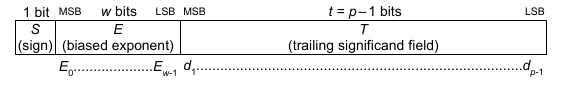
\includegraphics[width=0.45\textwidth]{IEEEinterchangeFormat.png}
 \caption{IEEE Interchange floating-point format \cite{4610935}}
 \label{IEEE_FLOAT}
\end{figure}
\begin{figure}[h!]
\centering
\begin{tabular}{|c|c|c|}
 \hline
 Precision & Exponent width & Significant precision \\
 \hline
 32-bit & 8 bits & 23 bits \\
 \hline
 64-bit & 11 bits & 52 bits \\
 \hline
\end{tabular}
\caption{Specifications for the 32-bit and 64-bit interchange formats}
 \label{IEEE_FLOAT_TAB}
\end{figure}
\subsection{Overview of predictive compression}
Previous research \cite{1607248,4589203,engelson2000lossless,lindstrom2006fast,O'Neil:2011:FDC:1964179.1964189,4976448} in this area has yielded good results both in terms of compression ratio and speed. 
The common line of thought is to predict successive values. Depending on the accuracy the difference between the predicted and actual value will hopefully be much smaller than the actual value itself. 
This difference can then be encoded using fewer bytes/bits of data (depending if compression occurs at a byte or bit level) by compressing the leading zeros after either an XOR or integer subtraction 
operation. Machine instructions to count the leading zeros can be found on AMD and newer Intel Processors. The leading zero count is then encoded as a prefix stream while the remaining bits/bytes 
are encoded as a residual stream.

Previous research suggests several different constructions of predictors. The use of a Lorenzo predictor \cite{lindstrom2006fast} generalizes a parallelogram predictor used by \cite{engelson2000lossless}. This
approach is particularly useful to compress large meshes of structures. Other approaches include the use of prediction history (via a simple lookup table construction) as suggested in \cite{1607248,4589203,4976448}. 
The later reports a throughput of up to 670 MB/s on a CPU implementation of their FPC compressor. An even simpler scheme \cite{O'Neil:2011:FDC:1964179.1964189} reportedly achieved throughputs of up to 75GB/s in its 
compression routine and up to 90GB/s in its decompression routine implemented in CUDA. In this scheme only the difference between successive values are encoded (this will clearly only work if the pairs of 
data points varies very little from one time step to the next). It is duly noted that the speeds achieved by \cite{O'Neil:2011:FDC:1964179.1964189} is on the post processing of results already stored in 
graphics memory. The implementations by \cite{O'Neil:2011:FDC:1964179.1964189,1607248,4589203,4976448,engelson2000lossless} targets 64-bit IEEE 754 \textit{double} precision floating-point data.

The primary scheme we propose takes its inspiration from \cite{O'Neil:2011:FDC:1964179.1964189}, but will operate on 32-bit IEEE 754 \textit{single} precision floating-point values. The uncompressed data itself 
is also structured slightly differently to the model used by \cite{O'Neil:2011:FDC:1964179.1964189}. Instead of compressing each consecutive value my compressor will compress consecutive blocks of data. Although 
the predictor itself is very simple and may not yield as good a compression ratio as the schemes suggested by the other authors it should obtain the required throughput. Additionally we will test the effectiveness
of a parallelogram predictor, a Lagrange extrapolation predictor \cite{engelson2000lossless} and a moving mean and median scheme. We will describe each implementation to greater extent in the implementation section.

As pointed out in previous research \cite{engelson2000lossless,lindstrom2006fast} using floating point operations in the prediction step can cause an irreversible loss of information due to floating point
rounding errors. A simple approach is proposed by \cite{engelson2000lossless}. Floating point memory is simply treated as integer memory and all operations performed on that memory are integer operations. This
approach assures us of achieving lossless compression and we will consequently only consider using schemes that conform to this approach. A simple case to illustrate this approach is made by \cite{engelson2000lossless}.
It is clearly visible in fig.~\ref{INT_REP} that if two floating-point numbers are relatively close to each other in terms of magnitude it is possible to discard some repeated bytes of information after performing 
an XOR operation to extract the remaining, seemingly random, residual bits. Therefore if we can accurately predict consecutive numbers we should be able to make reasonable
savings in terms of compression ratio.
\begin{figure}[h!]
\begin{tabular}{|c|c|c|c|}
 \hline
  & & byte & 1\hspace{8 pt}2\hspace{8 pt}3\hspace{8 pt}4\hspace{8 pt}5\hspace{8 pt}6\hspace{8 pt}7\hspace{8 pt}8\\
 \hline
 $a_{1}$ & 2.3667\textbf{1}76745585676 & $\Rightarrow$ & 40 02 ef \textbf{09 ad 18 c0 f6} \\
 \hline
 $a_{2}$ & 2.3667\textbf{2}76745585676 & $\Rightarrow$ & 40 02 ef \textbf{0e eb 46 23 2f} \\
 \hline
 $a_{3}$ & 2.3667\textbf{3}76745585676 & $\Rightarrow$ & 40 02 ef \textbf{14 29 73 85 6a} \\
 \hline
\end{tabular}
\caption{Treating 64-bit IEEE 754 double precision floating-points as integer memory \cite{engelson2000lossless}}
 \label{INT_REP}
\end{figure}
\subsection{Parallel prefix sums}
The computation of a prefix sum is a necessary step in the parallelization of a packing algorithm \cite{O'Neil:2011:FDC:1964179.1964189}. A prefix sum (or \textit{scan}) can 
be defined on any binary associative operator, $\oplus$ over an ordered set with $I$ as its identity. If $A=[a_{0},a_{1},\dots,a_{n-1}]$ is an ordered set then the prefix 
sum scan is defined as $scan(A):=[I,a_{0},(a_{0} \oplus a_{1}),\dots,(a_{0} \oplus a_{1} \oplus ... \oplus a_{n-2})]$.

This scan operation can be computed in parallel. Blelloch suggests such an approach in \cite{blelloch1990prefix}. We will discuss the algorithm in more detail in the section on implementation.
Additionally a work-efficient CUDA version of the algorithm is discussed in \cite{harris2007parallel}. In this version the algorithm is optimized to avoid bank conflicts and has been
shown to be 6 times faster than a sequential CPU implementation.
\section{Research questions}
We are investigating the feasibility of adding a \textit{online} predictive compression step to the existing KAT-7 / MeerKAT pipeline. Such a step has to meet at least two primary
criteria: high throughput and effective compression ratios. These are outlined below:
\begin{enumerate}
 \item Are predictive techniques fast enough? The algorithm should be able of achieving throughput rates of at least 40 GiB/s.
 \item Are predictive techniques effective? The algorithm should reduce the size of transmissions by several percent and hopefully
       this reduction can take the form of double digit figures. It has, however, been pointed out that the data may
       be too noisy to expect great reductions, while maintaining the throughput rate we mentioned above.
 \item Can throughput be traded for compression ratio using different predictors?
\end{enumerate}
\section{Design and Methodology}
\subsection{Packing algorithm}
The compacting algorithm we propose is based on the same approach taken by \cite{O'Neil:2011:FDC:1964179.1964189}. The algorithm is almost \textit{symetrical} in its compression and 
decompression stages. By symetrical we mean that  the algorithm is executed in the opposite direction when performing decompression. The primary difference is that we do not have to compute
the leading zero count of each element being decompressed. Refer to fig.~\ref{PACKING_ALGORITHM} for more details.

We use the construction specified in fig.~\ref{PACKING_ALGORITHM} because we can easily swap out one predictor for another. The predictor in this case can be any n-element predictor. As we mentioned
earlier the predicted value is XORed with the actual value to get a residual which can be compacted at either bit or byte level. This compaction simply removes the leading zeros from each residual and
store each as a fixed-length prefix count. We note that the number of bits needed to store $n$ leading zeros can be calculated as $\lfloor\log_2n\rfloor+1$ bits where $n\in\mathbb{N}_{>0}$. One aspact 
of this compression scheme that must be investigated is to determine which residual compaction scheme gives better results: packing at bit or byte level. Although a bit-packing scheme can pack
an arbitrary number of zeros it requires longer prefixes to store these counts. The opposite is true for byte-packing schemes. Since the prefixes are always short we use a bit-packing scheme to store
these fixed-length codes.
\begin{figure}[h!]
 \centering
 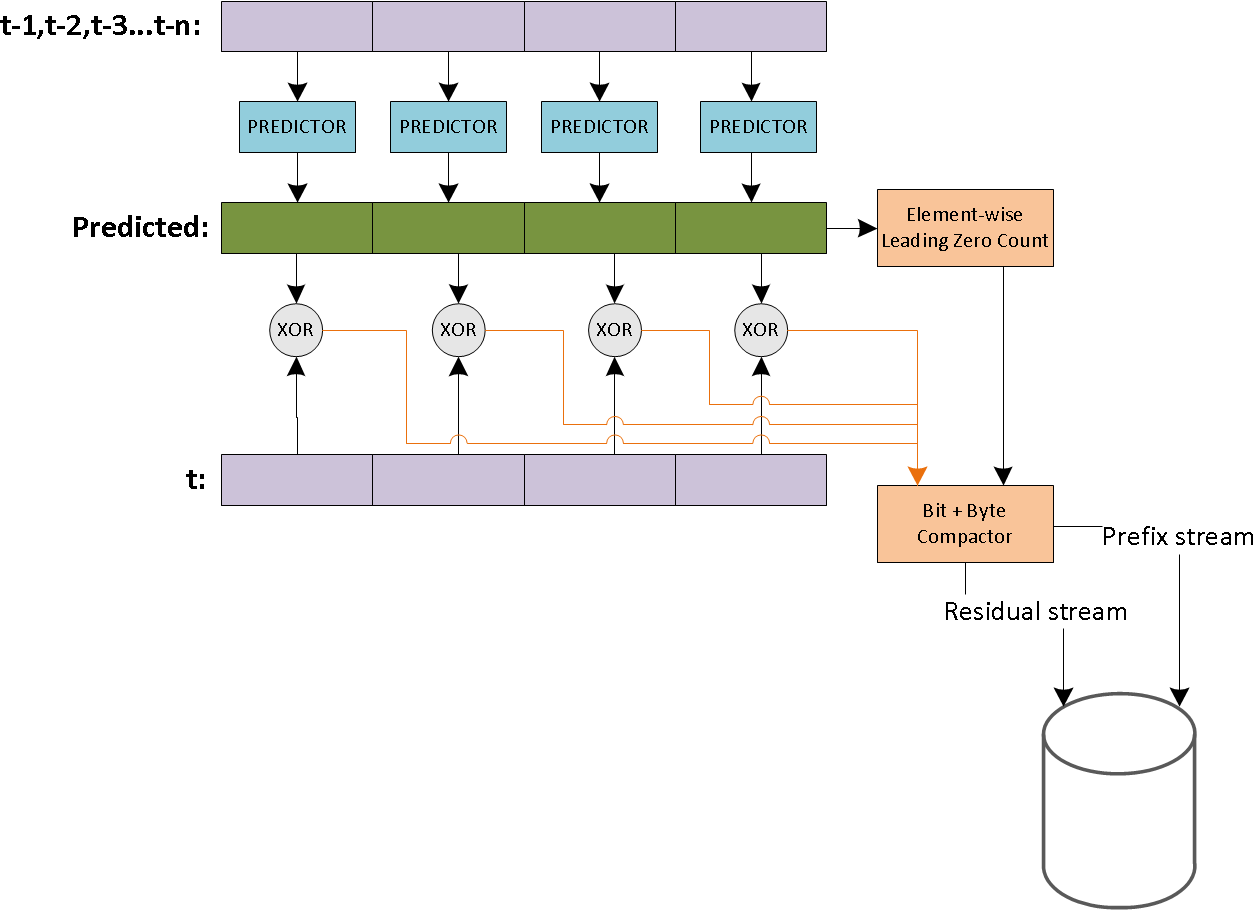
\includegraphics[width=0.50\textwidth]{Thesis_Alg.png}
 \caption{Prediction and compaction process}
 \label{PACKING_ALGORITHM}
\end{figure}
\subsection{Parallelizing compression and decompression steps}
We note that there are three ways this can be achieved: 
\begin{enumerate}
 \item Even though the residuals are of variable length it is possible to pack the them in parallel. However, it is duly noted that this adds an additional overhead to \textit{both} the packing and 
 unpacking process. The process requires a prefix sum to be computed for the array of element-wise leading zero counts. As we pointed out in the background chapter this prefix sum can be computed
 in parallel. After this the indexes have been accumulated using the prefix sum algorithm it is easy to see how different threads can pack residuals at the correct positions. We do, however, note that
 both a parallel bit and byte packing scheme will require atomic operations to ensure against the \textit{race condition} that arises when multiple threads writes to the same memory location 
 simultaneously. This memory-level-synchronization mechanism adds additional overhead in terms of wasted machine clock cycles.
 \item We can separate incoming data into blocks and do multiple of these blocks in parallel (where each block is compressed/decompressed in serial). This overcomes the issue of additional overheads arising
 from computing prefix sums and using atomics, but it should be noted that this approach may have a detrimental effect on the compression ratio since we have to store the length of the residual array of each block.
 We will have to investigate which of 1 or 2 yields better results for CPU implementations.
 \item A more fine-grained parallelization is possible using vectorized instructions. The various Intel SSE, Steaming SIMD (Single Instruction Multiple Data) instruction set extensions (up to version 4.2) provide
 us the opportunity to perform 4 instructions (adds, multiplies, logarithms, rounding, etc.) simultaneously per core. However, the SSE instruction sets do not have any element-wise bit-shift operations. We propose 
 using a combination of the Intel SSE and AMD XOP instruction sets to achieve our goal. The XOP instruction set extends the SSE instruction set by adding these operations as one of its primary features. It should
 be duly noted that adding these instructions make the implementation dependent on the architecture of the machine it is executed on (and therefore less portable). If this approach is successful we recommend 
 that the vectorized code be extended to use the latest Intel AVX 2 instruction set in which Intel introduces element-wise shift operations and offset-loading operations. The AVX family of instructions
 can compute up to 8 SIMD operations in parallel per core. It is duly noted that these instruction sets make use of a very limited number of 128- and 256-bit registers respectively. We will need to investigate
 whether it is worthwhile to implement the proposed packing algorithm using these instructions.
\end{enumerate}
\subsection{Porting the implementation to CUDA}
General Purpose programming using Graphics Processing Units (GPGPU) brings a host of associated challenges. These challenges arise primarily due to the widely differing architecture of GPUs compared (if compared
with the classical architectures of Central Processing Units, CPUs). Refer to fig.~\ref{FERMI_ARCH} for a detailed overview of the microchip die structure of a Nvidia Fermi generation GPU. It is also worthwhile to note 
that each generation of GPUs have varying architectures, making many optimizations architecture specific. Each generation, for instance, will have a different ratio and configuration of arithmetic cores to floating point
and special operations cores per group of processing \textit{CUDA cores} also known as \textit{SMs} or \textit{SMXs} on the latest \textit{Kepler} generation. Each generation also have widely differing memory 
controller properties. These may determine how many warps of cores can be executed, when the warps are swapped in/out, along with many others. 

We will provide a basic CUDA implementation to see if doing compression as a post-processing step on signal data already loaded to GPU as part of the current pipeline is a feasible alternative to a regular 
multi-threaded CPU implementation. We will make use of shared memory and our implementation will take adequate precaution to coalesce memory accesses and to avoid bank conflicts when possible. More details 
will be provided in the implementation section, but it is clear that a combination of the approaches (1 \& 2) taken with the CPU version will be required to make adequate use of the GPU architecture. Our 
implementation will consider assigning a block of data to each SM, which will in turn process that block in parallel without regard to operations performed on other SMs. This ensures that we do not create 
unnecessary overhead synchronizing SMs (this is considered to be a very costly synchronization for this type of architecture). Instead all atomic operations and synchronization steps will be performed on a 
per-SM basis only.
\begin{figure}[h!]
 \centering
 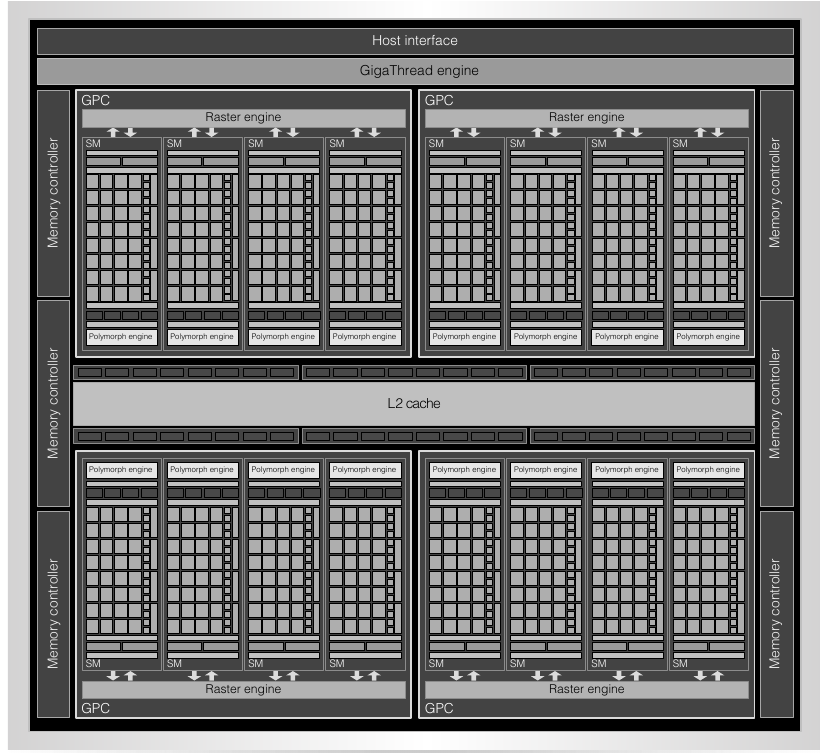
\includegraphics[width=0.50\textwidth]{fermi_arch.png}
 \caption{Architecture of the Fermi family of Nvidia GPUs \cite{wittenbrink2011fermi}}
 \label{FERMI_ARCH}
\end{figure}
\subsection{Test data}
{\color{red}TODO}
\subsection{Benchmarks}
{\color{red}TODO}
\subsection{Benchmarking platform}
{\color{red}TODO}
\section{Implementation}
{\color{red}TODO}
\section{Findings}
{\color{red}TODO}
\section{Discussion}
{\color{red}TODO}
\section{Conclusion}
{\color{red}TODO}
\section{Future avenues of research}
{\color{red}TODO}
\section{Acknowledgements}
I would like to acknowledge A/Prof. James Gain and Dr. Patrick Marais of the Department of Computer Science at the University of Cape Town for their continuous, expert, input on the project.

Secondly I would like to thank Jason Manley, a Digital Signals Processing specialist at the MeerKAT offices in Pinelands, Cape Town for providing us with technical information
on the MeerKAT project. Jason has also kindly prepared a 100 GB of sample of KAT-7 output data for testing purposes.

Thirdly I would like to note that all tests were performed on the ICTS High Performance (\textit{HEX}) cluster at the University of Cape Town. The cluster has 4 DELL C6145 nodes each boasting 4 16-core
AMD Opteron 6274 CPUs, clocked at 2200 MHz with 16 MB L3 cache memory. There are two additional GPU nodes with 4 Tesla M2090 GPU cards each. Each GPU card has 6 GB GDDR5 and 2048 CUDA cores. I want to 
especially thank Andrew Lewis from ICTS for his assistance and support during testing.

This research is made possible under grant of the National Research Foundation (hereafter \textit{NRF}) of the Republic of South Africa. All views expressed in this report are those of the author and not the NRF.
\bibliographystyle{plain}
\bibliography{litRefs}
\end{document}
